

\subsection{Rango de tiempo}
\begin{table}[H]
\centering
\begin{tabular}{c|c|c}
Inicio & 1388628499 & 2 January 2014 \\ \hline
Final  & 1550534100 & 18 February 2019 \\
\end{tabular}
\end{table}

\subsection{Tasa de eventos}

\begin{figure}[H]
	\centering
	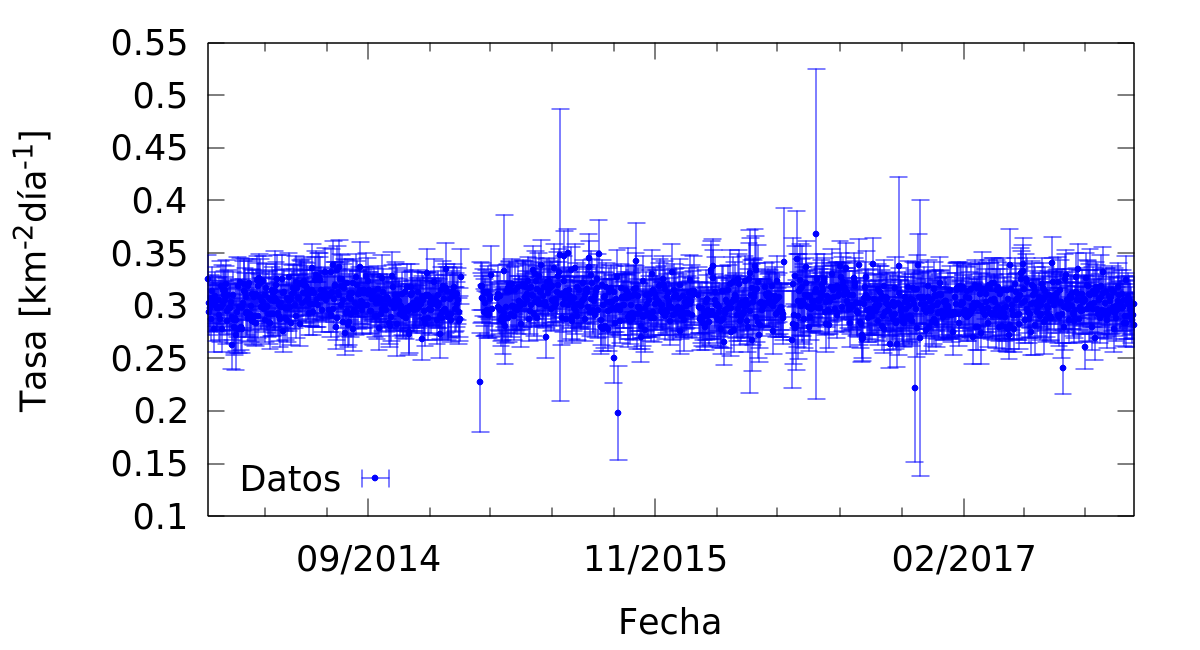
\includegraphics[width=0.5\textwidth]{rate_1_EeV.png}
	\caption{Tasa de eventos para eventos por encima de 1 EeV.}
\end{figure}

Antes del 2 de Enero del 2014, se tenía una tasa por debajo de la media de los siguientes años.

La cantidad de hexágonos 6T5 durante el periodo mencionado arriba evolucionó como se muestra  en la figura que sigue


\begin{figure}[H]
	\centering
	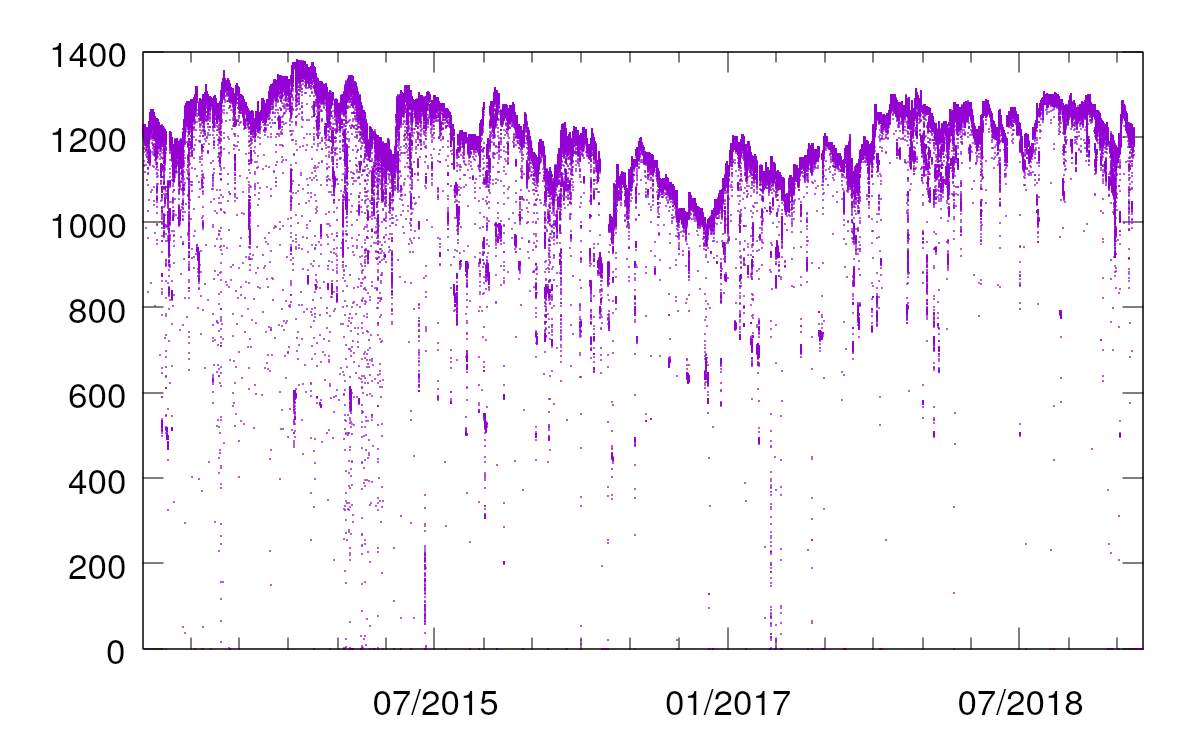
\includegraphics[width=0.5\textwidth]{hex_rango_corto.png}
	\caption{Hexágonos}
\end{figure}


\subsection{Párametros del clima}

\begin{figure}[H]
	\centering
	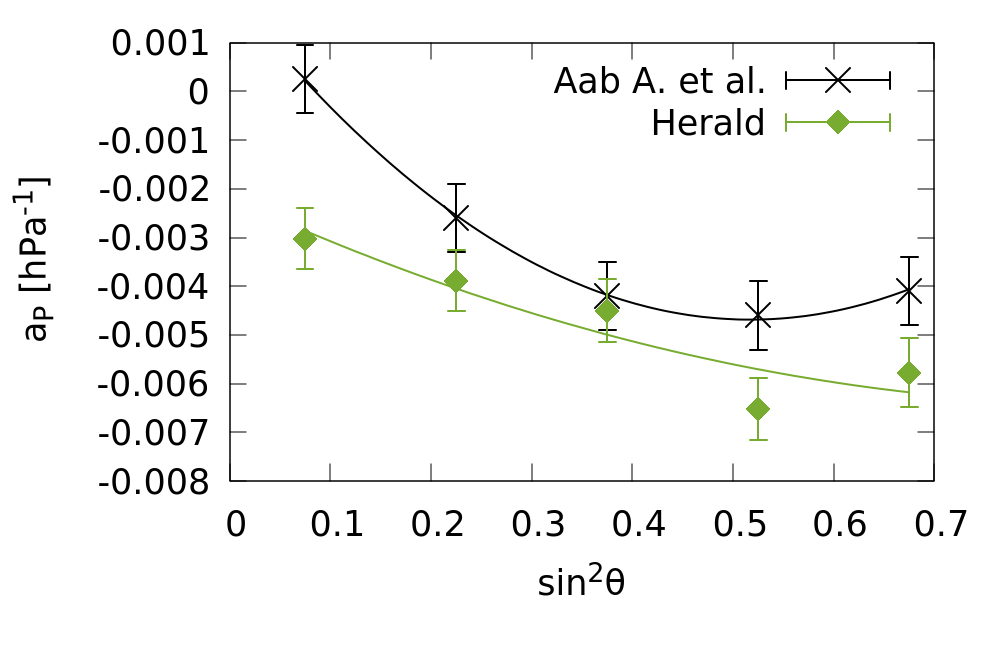
\includegraphics[width=0.5\textwidth]{ap.png}
\end{figure}


\begin{figure}[H]
	\centering
	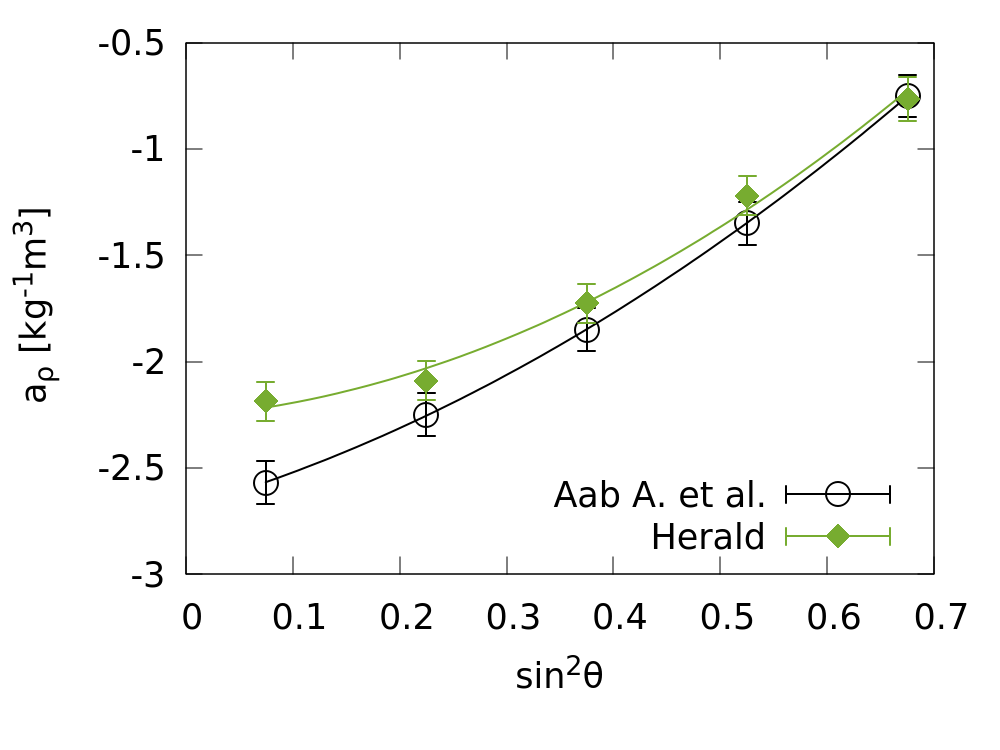
\includegraphics[width=0.5\textwidth]{arho.png}
\end{figure}


\begin{figure}[H]
	\centering
	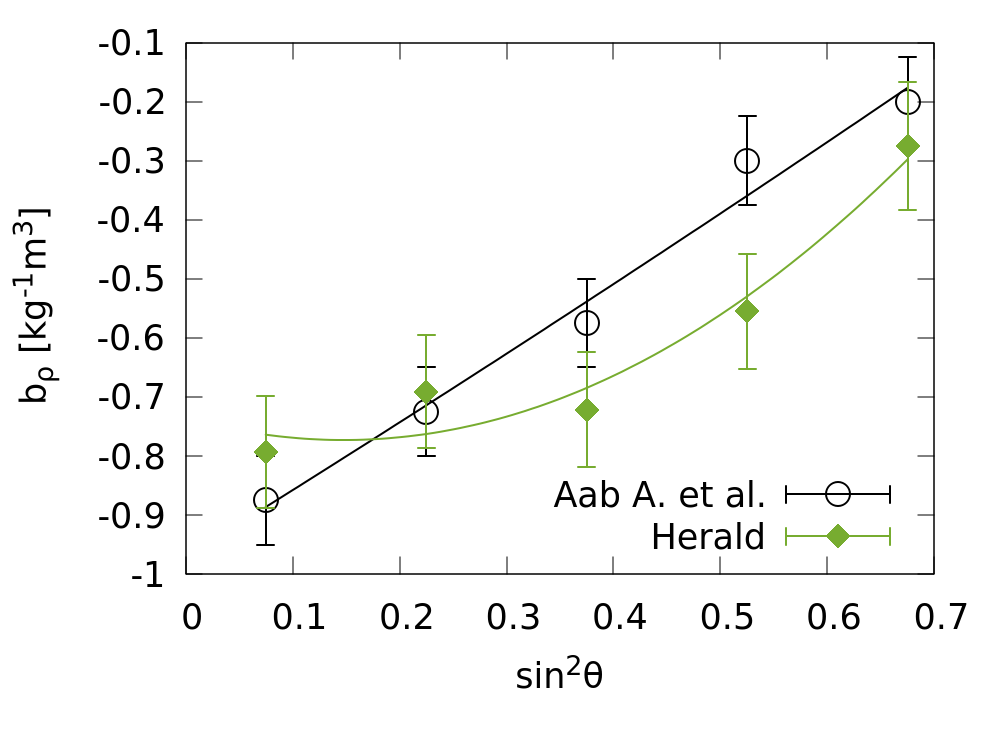
\includegraphics[width=0.5\textwidth]{brho.png}
\end{figure}




Considerando una cuádrica para el ajuste de la curva, se obtiene los parámetros de la siguiente table
\begin{table}[H]
\centering
\begin{tabular}{c|c|c|c}
		 	& $a_P$ 	&  $a_\rho$  & $ b_\rho$ \\ \hline
$c_0$ 		& -0.002(1) & 	-2.2(1)	 &	-0.74(9)\\ \hline
$c_1$ 		& -0.009(6)	& 	 0.4(6)	 &	-0.0(6)\\ \hline
$c_2$ 		&  0.00(9) 	& 	 2.7(8)  &	 1.7(7)\\ \hline
\end{tabular}
\end{table}


\subsection{Anisotropía en el rango 1-2 EeV}

\begin{figure}[htbp]
	\centering
	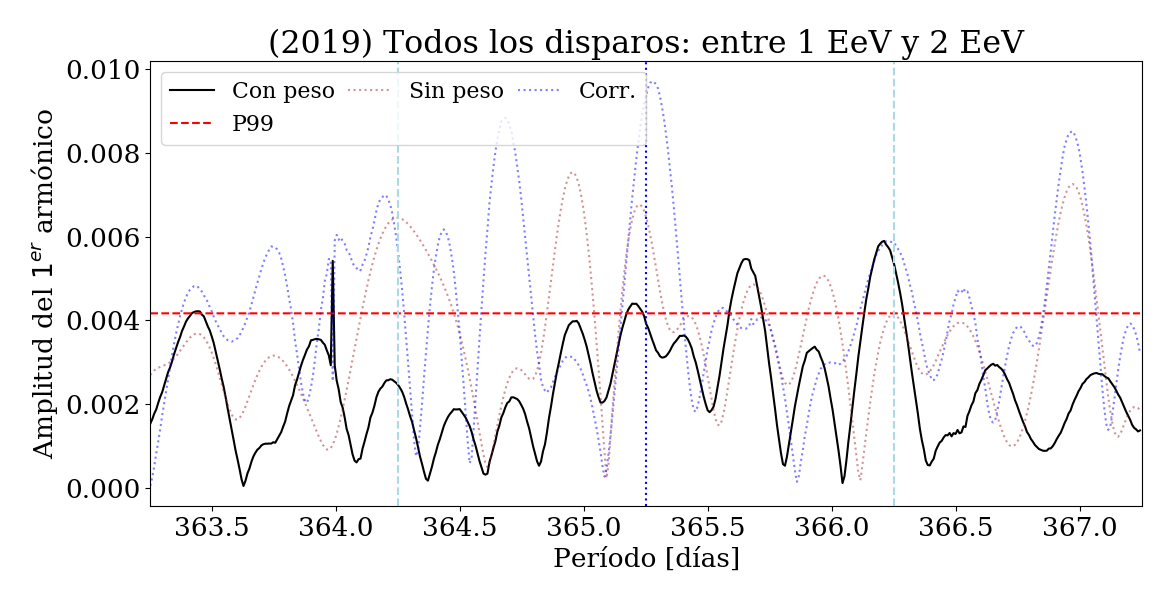
\includegraphics[width=0.5\textwidth]{ani_corr.png}
\end{figure}






\section{Introducción}

 %{Introducción}

\begin{itemize}
  \item Cosas que hice en la tesis de licenciatura.
  \begin{itemize}
  	\item[-] Corrección del clima
  	\item[-] Familiarizarse con el dataset
  \end{itemize}
  \item Resultados a los que llegué.
  \item Nos movimos a otros disparos (MoP y ToTs)
\end{itemize}

 

 %{Introducción}

\begin{figure}[htbp]
  \centering
  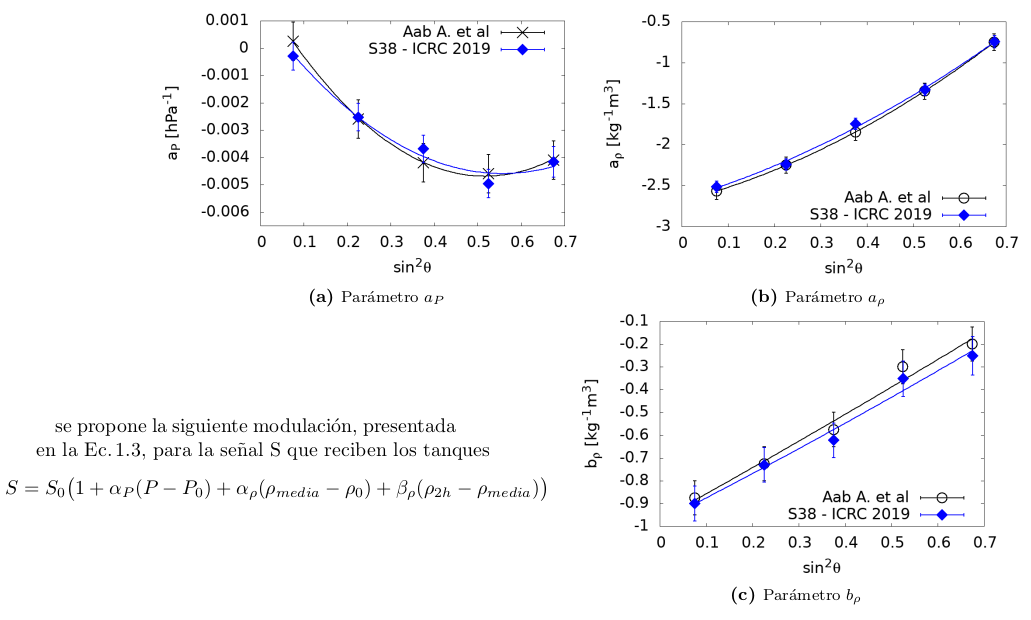
\includegraphics[width=0.95\textwidth]{../beamer-07-05-2020/tesis.png}
\end{figure}

 

\section{Update}

 %{Update}

  \begin{itemize}
  	\item Diferencias con el disparo tradicional.
    \begin{itemize}
      \item[-] Empieza en el 2013
      \item[-] Eficiencia
      \item[-] Cantidad de datos en el bin de 1 EeV - 2 EeV.
    \end{itemize}
  	\item Pesos de los hexágonos.
  	\item Resultados con el rango de energía 1 EeV - 2 EeV.
    \item ¿Podemos mejorarlo con la corrección del clima?
  \end{itemize}


 


\subsection{Cálculo de Rayleigh.}

 %{Pesos}
 %{Cálculo de Rayleigh: ¿Por qué importan los pesos?}

 \begin{enumerate}
   \item Fijo una frecuencia a estudiar.
   \item Me muevo en el dataset de hexagonos, a cada utc lo clasifico según:
   \begin{equation*}
     h = (\text{hora local })\times \nicefrac{\text{Frecuencia a estudiar}}{\text{Frecuencia Solar}}
   \end{equation*}
     \item El valor de h no es continuo, sino está divido en 288 segmentos entre 1 y 24
  \item Le asigno un peso al bin h:
   \begin{align*}
     \text{peso del bin h} &= \nicefrac{\text{Hexagonos que cayeron en el bin h}}{I}\\
     I &= \sum^{288}_h \nicefrac{\text{Hexagonos que cayeron en el bin h}}{288}
    \end{align*} 

 \end{enumerate}

 



\subsection{Pesos de los hexágonos}

 %{Pesos}
 %{Pesos de los hexágonos}

\begin{figure}[htbp]
  \centering
  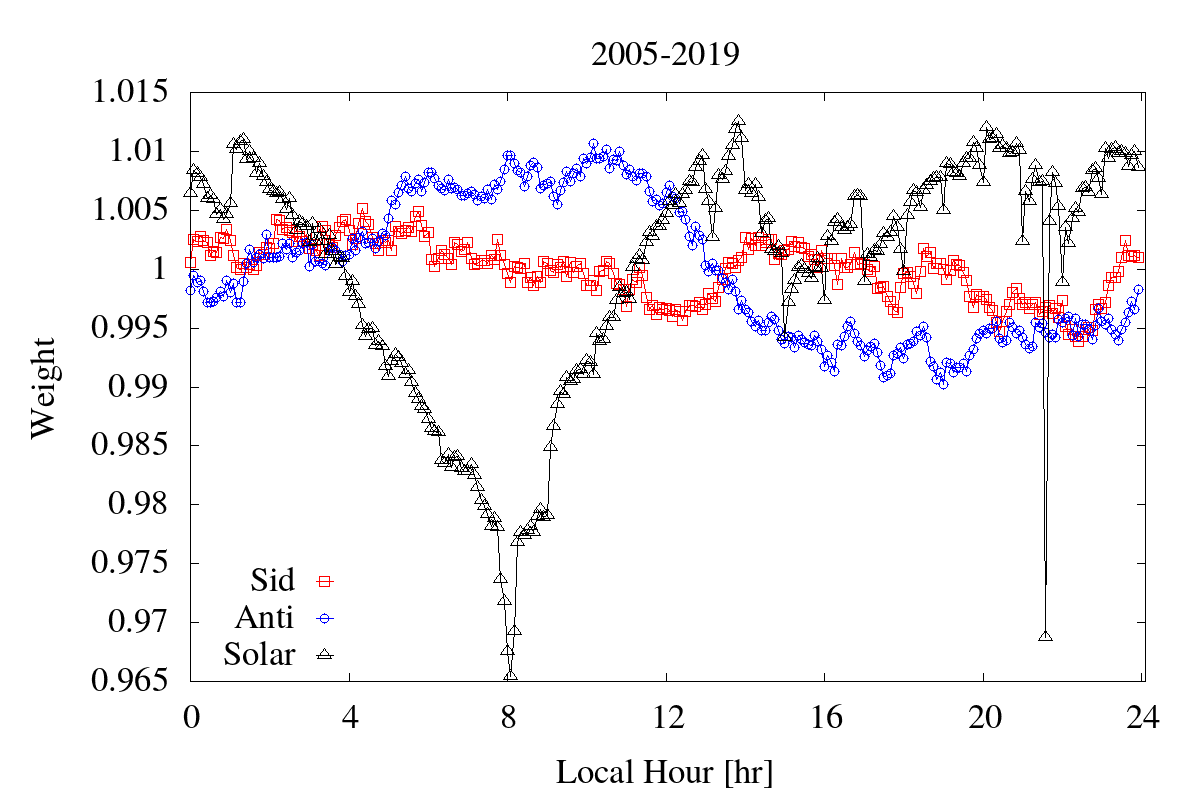
\includegraphics[width=0.95\textwidth]{../report_2_27_04_2020/Graficos/weigth2005-2019.png}
  \caption{Un ejemplo de pesos de los hexágonos en el rango 2005-2019 para distintas frecuencias.}
\end{figure}

 

 %{Pesos}
 %{Pesos de los hexágonos}

\begin{figure}[htbp]
  \centering
  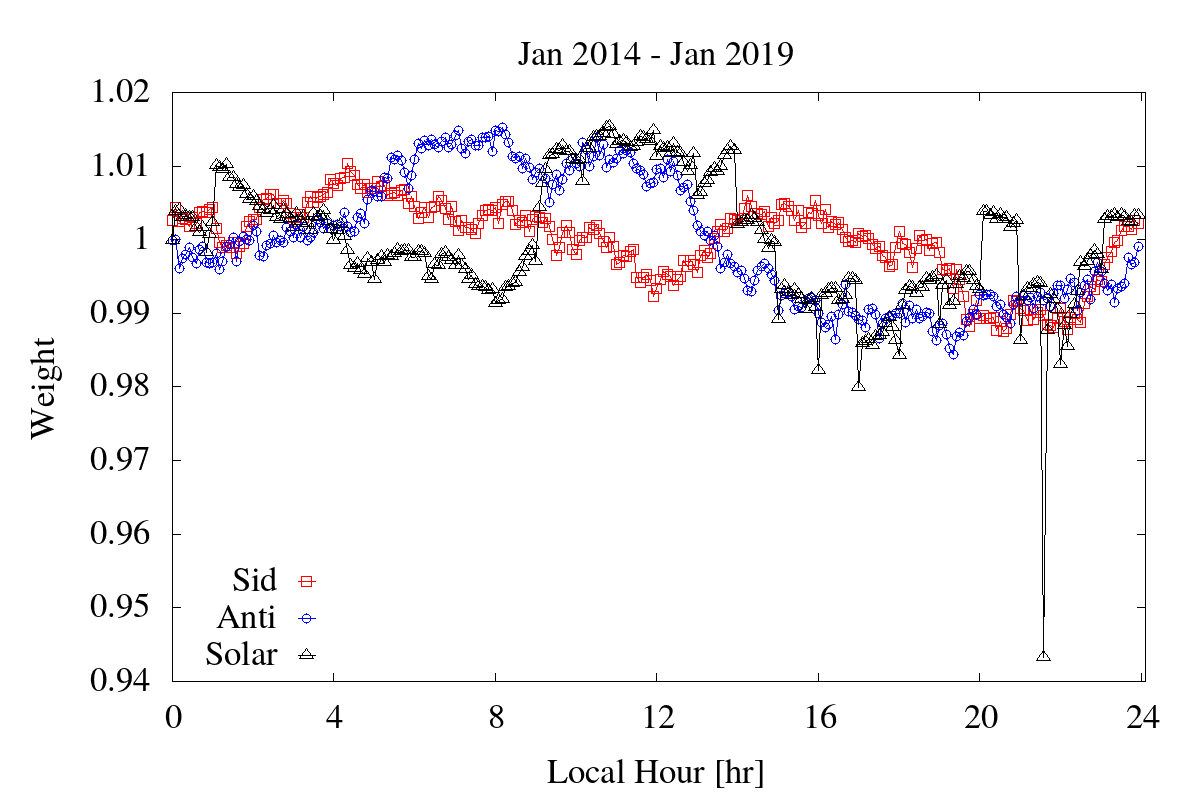
\includegraphics[width=0.95\textwidth]{../../Plotting/weigth2014-2019_jan.png}
  \caption{Un ejemplo de pesos de los hexágonos en el rango Enero 2014- Enero 2019 para distintas frecuencias.}
\end{figure}

 



\subsection{Cálculo de Rayleigh.}

 %{Pesos}
 %{Cálculo de Rayleigh: ¿Por qué importan los pesos?}

 \begin{enumerate}
   \item Fijo una frecuencia a estudiar.
   \item Me muevo en el cielo con esa frecuencia (fase).
   \item Dado el utc del evento, lo clasifico según:
   \begin{equation*}
     h = (\text{hora local })\times \nicefrac{\text{Frecuencia a estudiar}}{\text{Frecuencia Solar}}
   \end{equation*}
     \item El valor de h no es continuo, sino está divido en 288 segmentos entre 1 y 24
  \item Le asigno un peso por evento:
   \begin{equation*}
     \text{peso del evento} = (\text{peso  de los hexágonos para el bin h})^{-1}
     \end{equation*} 
    \item Hago el análisis en frecuencias:
    \begin{align*}
        a &= \sum^{Eventos}_i \cos(2\pi \nicefrac{h}{24} + (RA -RA_{cenit}))\times \nicefrac{(\text{peso del evento})_i}{N}\\
        b &= \text{Lo mismo pero con seno}\qquad         N = \sum^{Eventos}_i \text{peso del evento}_i
    \end{align*}
 \end{enumerate}

 



\subsection{Resultados con el rango de energía 1 EeV - 2 EeV}


 %{Bin 1EeV-2EeV}
 %{Resultados con el rango de energía 1 EeV - 2 EeV}

\begin{figure}[htbp]
  \centering
  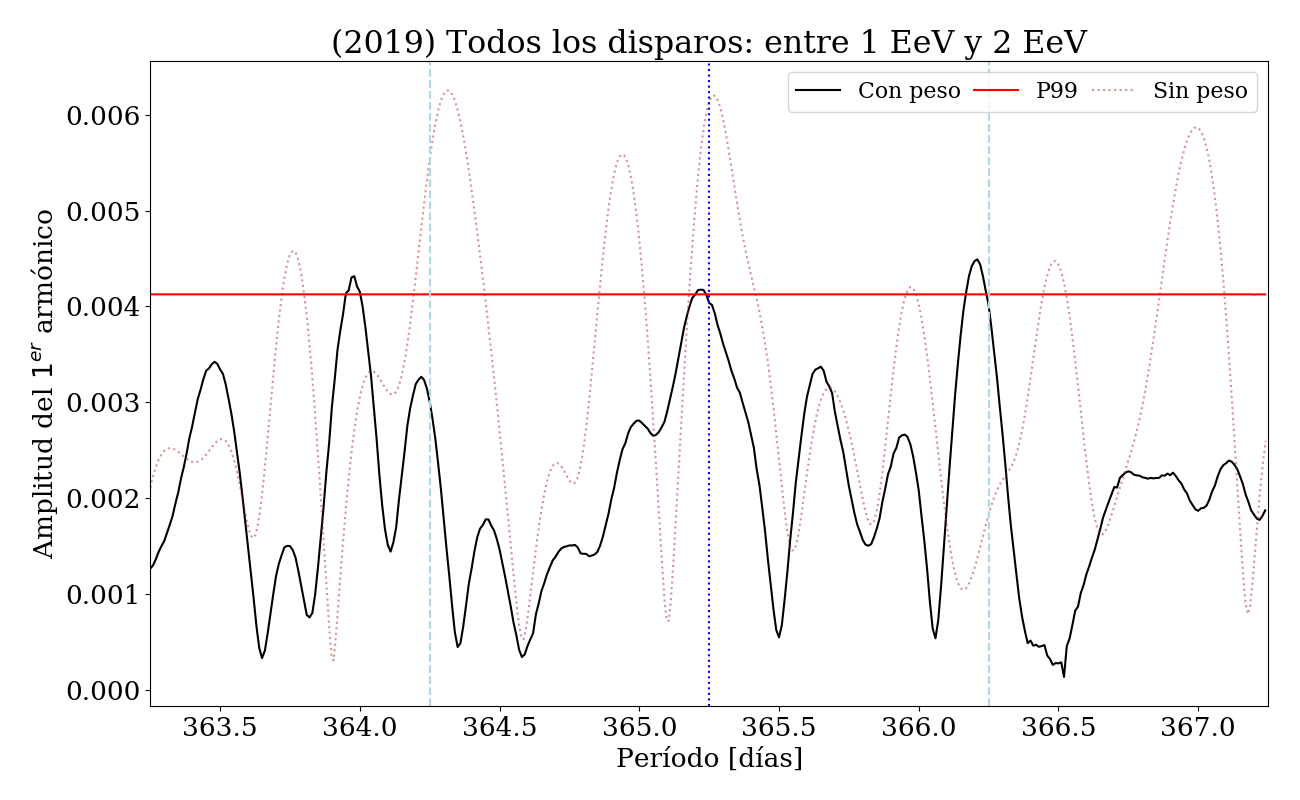
\includegraphics[width=\textwidth]{./../../Python/xx2019_AllTriggers_1_2_EeV_con_vs_sin_peso.png}
  \caption{Análisis en frecuencia para el bin 1 EeV - 2 EeV, entre Enero 2014- Enero 2019 (Cantidad de eventos $ \approx 10^6$).}
\end{figure}

 



